% Options for packages loaded elsewhere
\PassOptionsToPackage{unicode}{hyperref}
\PassOptionsToPackage{hyphens}{url}
\PassOptionsToPackage{dvipsnames,svgnames,x11names}{xcolor}
%
\documentclass[
12pt]{article}

\usepackage{amsmath,amssymb}
\usepackage{iftex}
\ifPDFTeX
\usepackage[T1]{fontenc}
\usepackage[utf8]{inputenc}
\usepackage{textcomp} % provide euro and other symbols
\else % if luatex or xetex
\usepackage{unicode-math}
\defaultfontfeatures{Scale=MatchLowercase}
\defaultfontfeatures[\rmfamily]{Ligatures=TeX,Scale=1}
\fi
\usepackage{lmodern}
\ifPDFTeX\else  
% xetex/luatex font selection
\fi
% Use upquote if available, for straight quotes in verbatim environments
\IfFileExists{upquote.sty}{\usepackage{upquote}}{}
\IfFileExists{microtype.sty}{% use microtype if available
	\usepackage[]{microtype}
	\UseMicrotypeSet[protrusion]{basicmath} % disable protrusion for tt fonts
}{}
\makeatletter
\@ifundefined{KOMAClassName}{% if non-KOMA class
	\IfFileExists{parskip.sty}{%
		\usepackage{parskip}
	}{% else
		\setlength{\parindent}{0pt}
		\setlength{\parskip}{6pt plus 2pt minus 1pt}}
}{% if KOMA class
	\KOMAoptions{parskip=half}}
\makeatother
\usepackage{xcolor}
\setlength{\emergencystretch}{3em} % prevent overfull lines
\setcounter{secnumdepth}{5}
% Make \paragraph and \subparagraph free-standing
\makeatletter
\ifx\paragraph\undefined\else
\let\oldparagraph\paragraph
\renewcommand{\paragraph}{
	\@ifstar
	\xxxParagraphStar
	\xxxParagraphNoStar
}
\newcommand{\xxxParagraphStar}[1]{\oldparagraph*{#1}\mbox{}}
\newcommand{\xxxParagraphNoStar}[1]{\oldparagraph{#1}\mbox{}}
\fi
\ifx\subparagraph\undefined\else
\let\oldsubparagraph\subparagraph
\renewcommand{\subparagraph}{
	\@ifstar
	\xxxSubParagraphStar
	\xxxSubParagraphNoStar
}
\newcommand{\xxxSubParagraphStar}[1]{\oldsubparagraph*{#1}\mbox{}}
\newcommand{\xxxSubParagraphNoStar}[1]{\oldsubparagraph{#1}\mbox{}}
\fi
\makeatother


\providecommand{\tightlist}{%
	\setlength{\itemsep}{0pt}\setlength{\parskip}{0pt}}\usepackage{longtable,booktabs,array}
\usepackage{calc} % for calculating minipage widths
% Correct order of tables after \paragraph or \subparagraph
\usepackage{etoolbox}
\makeatletter
\patchcmd\longtable{\par}{\if@noskipsec\mbox{}\fi\par}{}{}
\makeatother
% Allow footnotes in longtable head/foot
\IfFileExists{footnotehyper.sty}{\usepackage{footnotehyper}}{\usepackage{footnote}}
\makesavenoteenv{longtable}
\usepackage{graphicx}
\makeatletter
\def\maxwidth{\ifdim\Gin@nat@width>\linewidth\linewidth\else\Gin@nat@width\fi}
\def\maxheight{\ifdim\Gin@nat@height>\textheight\textheight\else\Gin@nat@height\fi}
\makeatother
% Scale images if necessary, so that they will not overflow the page
% margins by default, and it is still possible to overwrite the defaults
% using explicit options in \includegraphics[width, height, ...]{}
\setkeys{Gin}{width=\maxwidth,height=\maxheight,keepaspectratio}
% Set default figure placement to htbp
\makeatletter
\def\fps@figure{htbp}
\makeatother

\addtolength{\oddsidemargin}{-.5in}%
\addtolength{\evensidemargin}{-.1in}%
\addtolength{\textwidth}{1in}%
\addtolength{\textheight}{1.7in}%
\addtolength{\topmargin}{-1in}
\makeatletter
\@ifpackageloaded{caption}{}{\usepackage{caption}}
\AtBeginDocument{%
	\ifdefined\contentsname
	\renewcommand*\contentsname{Table of contents}
	\else
	\newcommand\contentsname{Table of contents}
	\fi
	\ifdefined\listfigurename
	\renewcommand*\listfigurename{List of Figures}
	\else
	\newcommand\listfigurename{List of Figures}
	\fi
	\ifdefined\listtablename
	\renewcommand*\listtablename{List of Tables}
	\else
	\newcommand\listtablename{List of Tables}
	\fi
	\ifdefined\figurename
	\renewcommand*\figurename{Figure}
	\else
	\newcommand\figurename{Figure}
	\fi
	\ifdefined\tablename
	\renewcommand*\tablename{Table}
	\else
	\newcommand\tablename{Table}
	\fi
}
\@ifpackageloaded{float}{}{\usepackage{float}}
\floatstyle{ruled}
\@ifundefined{c@chapter}{\newfloat{codelisting}{h}{lop}}{\newfloat{codelisting}{h}{lop}[chapter]}
\floatname{codelisting}{Listing}
\newcommand*\listoflistings{\listof{codelisting}{List of Listings}}
\makeatother
\makeatletter
\makeatother
\makeatletter
\@ifpackageloaded{caption}{}{\usepackage{caption}}
\@ifpackageloaded{subcaption}{}{\usepackage{subcaption}}
\makeatother


\ifLuaTeX
\usepackage{selnolig}  % disable illegal ligatures
\fi
\usepackage[]{natbib}
\bibliographystyle{agsm}
\usepackage{bookmark}

\IfFileExists{xurl.sty}{\usepackage{xurl}}{} % add URL line breaks if available
\urlstyle{same} % disable monospaced font for URLs
\hypersetup{
	pdftitle={Title},
	pdfauthor={Author 1; Author 2},
	pdfkeywords={3 to 6 keywords, that do not appear in the title},
	colorlinks=true,
	linkcolor={blue},
	filecolor={Maroon},
	citecolor={Blue},
	urlcolor={Blue},
	pdfcreator={LaTeX via pandoc}}

\usepackage{mathtools}
\usepackage{amssymb}
\usepackage{amsmath}
\usepackage{bigints}
\usepackage{algpseudocode}
\usepackage{algorithm}
\usepackage{amsthm}
\usepackage{soul}
\usepackage{makecell}
\usepackage[capitalise]{cleveref}
\usepackage{subcaption}
\newtheorem{theorem}{Theorem}[section]
\newtheorem{corollary}{Corollary}[section]
\newtheorem{lemma}{Lemma}[section]
\newtheorem{definition}{Definition}[section]
\newtheorem{assumption}{Assumption}[section]
\renewcommand{\theassumption}{\arabic{assumption}}
\newtheorem{manualtheoreminner}{Theorem}
\newenvironment{manualtheorem}[1]{%
	\IfBlankTF{#1}
	{\renewcommand{\themanualtheoreminner}{\unskip}}
	{\renewcommand\themanualtheoreminner{#1}}%
	\manualtheoreminner
}{\endmanualtheoreminner}

%
\usepackage{tikz}
\usetikzlibrary{arrows.meta, shapes.multipart, positioning, calc}

\tikzset{
	treenode/.style={
		rectangle, draw=black, rounded corners, minimum width=16mm, minimum height=8mm,
		align=center, font=\footnotesize
	},
	term/.style={treenode, fill=gray!10},
	internal/.style={treenode, fill=blue!5},
	edge/.style={-Latex, line width=1pt},
	oplabel/.style={font=\small\bfseries}
}


\newcommand{\anon}{1}

%set the key \texttt{anon} to ``0'' to hide the authors and acknowledgements,
%  producing the required anonymized version. 
%Set the key \texttt{anon} to ``1'' to produce the manuscript with author details and
% acknowledgments. 

\begin{document}


\def\spacingset#1{\renewcommand{\baselinestretch}%
{#1}\small\normalsize} \spacingset{1}


%%%%%%%%%%%%%%%%%%%%%%%%%%%%%%%%%%%%%%%%%%%%%%%%%%%%%%%%%%%%%%%%%%%%%%%%%%%%%%


\if1\anon
{
  \title{\bf Supplementary Material to Conditional Copula models using loss-based Bayesian Additive Regression Trees}
  \author{Tathagata Basu\thanks{
    The authors gratefully acknowledge Leverhulme Trust for funding this research (Grant RPG-2022-026)}\hspace{.2cm}\\
    Newcastle University, UK\\
    and \\
    Fabrizio Leisen \\
    Kings College London, UK\\
    and \\
    Cristiano Villa \\
    Duke Kunshan University, China\\
    and \\
    Kevin Wilson \\
    Newcastle University, UK}
  \maketitle
} \fi

\if0\anon
{
  \bigskip
  \bigskip
  \bigskip
  \begin{center}
    {\LARGE\bf Supplementary Material to Conditional Copula models using loss-based Bayesian Additive Regression Trees}
\end{center}
  \medskip
} \fi


\section{Description of the RJ-MCMC algorithm}\label{app:rj-mcmc}

We define our reversible jump MCMC algorithm based on the tree MCMC algorithm suggested by \cite{chipman98BCART} coupled with the generation of new terminal node values such that for the $k$-th tree at the $\eta$-th iteration, the proposal can be written in the following way:
\begin{align}\label{eq:prop}
	q\left(T_k^{\eta},M_k^{\eta};T_k^{\ast}, M_k^{\ast}\right) = q\left(T_k^{\eta};T_k^{\ast}\right) q_{\left(T_k^{\eta};T_k^{\ast}\right)}\left(M_k^{\eta};M_k^{\ast}\right).
\end{align}

For each tree $T$, we associate four different sets of nodes that are crucial for tree MCMC algorithm. 

\begin{itemize}
	\item $\mathcal{TN}(T_k)$: the set of all terminal nodes of a tree
	\item $\mathcal{IN}(T_k)$: the set of internal nodes
	\item $\mathcal{PN}(T_k)$: the set of all prunable nodes. That is all internal nodes which have two terminal nodes as children
	\item $\mathcal{PCN}(T_k)$: the set of all internal parent-child pairs.
\end{itemize}

To sample a new tree, we use four different tree moves \textsc{grow}, \textsc{prune}, \textsc{change} and \textsc{swap}. We define these moves in the following way:

\begin{itemize}
	\item \textsc{grow}: We randomly choose a terminal node $j$ from $\mathcal{TN}(T_k)$ and grow it to two different terminal nodes $j_l$ and $j_r$ with splitting rule $x\le c$ sampled from $\pi_{\textsc{rule}}(l\mid c)$. 
	\item \textsc{prune}: We randomly choose an internal node $j$ from $\mathcal{PN}(T_k)$ and delete its children.
	\item \textsc{change}: We randomly choose an internal node $j$ from $\mathcal{IN}(T_k)$ and assign a new splitting rule.
	\item \textsc{swap}: We randomly choose a parent-child pair $(a,b)$ from $\mathcal{PCN}(T_k)$ and swap their splitting rules.
\end{itemize}
We illustrate these tree MCMC moves in \cref{fig:tree:MCMC}.

\begin{figure}[h]
	\centering
	\begin{subfigure}{\textwidth}
		\centering
		\begin{tikzpicture}[every node/.style={font=\footnotesize}]
			%----------------------------------
			% Left tree
			%----------------------------------
			\begin{scope}[shift={(-4.5cm,0)}] % adjust -4.5cm based on tree width
				\node (left) {
					\begin{tikzpicture}[
						level 1/.style={level distance=8mm, sibling distance=40mm},
						level 2/.style={level distance=8mm, sibling distance=20mm},
						treenode/.style={rectangle, draw=black, rounded corners,
							minimum width=14mm, minimum height=6mm, align=center},
						internal/.style={treenode, fill=blue!10},
						term/.style={treenode, fill=gray!10}]
						\node[internal] {$x_1 < c_1$}
						child { node[internal] {$x_2 < c_2$}
							child { node[term] {$\mu_1$} }
							child { node[term] {$\mu_2$} }
						}
						child { node[term] {$\mu$} };
					\end{tikzpicture}
				};
			\end{scope}
			
			%----------------------------------
			% Arrow at origin
			%----------------------------------
			\node at (0,0) {\Huge$\Longrightarrow$};
			
			%----------------------------------
			% Right tree
			%----------------------------------
			\begin{scope}[shift={(4.5cm,0)}] % adjust 4.5cm based on tree width
				\node (right) {
					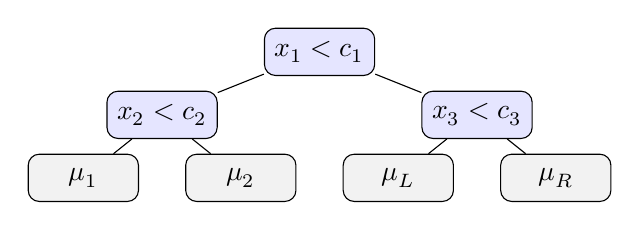
\begin{tikzpicture}[
						level 1/.style={level distance=8mm, sibling distance=40mm},
						level 2/.style={level distance=8mm, sibling distance=20mm},
						treenode/.style={rectangle, draw=black, rounded corners,
							minimum width=14mm, minimum height=6mm, align=center},
						internal/.style={treenode, fill=blue!10},
						term/.style={treenode, fill=gray!10}]
						\node[internal] {$x_1 < c_1$}
						child { node[internal] {$x_2 < c_2$}
							child { node[term] {$\mu_1$} }
							child { node[term] {$\mu_2$} }
						}
						child { node[internal] {$x_3 < c_3$}
							child { node[term] {$\mu_L$} }
							child { node[term] {$\mu_R$} }
						};
					\end{tikzpicture}
				};
			\end{scope}
		\end{tikzpicture}
		\caption{Original tree (left) and grown tree (right).}
	\end{subfigure}
	
	\begin{subfigure}{\textwidth}
		\centering
		\begin{tikzpicture}[every node/.style={font=\footnotesize}]
			%----------------------------------
			% Arrow at origin
			%----------------------------------
			\node (arrow) at (0,0) {\Huge$\Longrightarrow$};
			
			%----------------------------------
			% Left tree (shifted left)
			%----------------------------------
			\begin{scope}[shift={(-4.5cm,0)}] % adjust -5cm based on left tree width
				\node {
					\begin{tikzpicture}[
						level 1/.style={level distance=8mm, sibling distance=40mm},
						level 2/.style={level distance=8mm, sibling distance=20mm},
						treenode/.style={rectangle, draw=black, rounded corners, minimum width=14mm, minimum height=6mm, align=center},
						internal/.style={treenode, fill=blue!10},
						term/.style={treenode, fill=gray!10}]
						\node[internal] {$x_1 < c_1$}
						child { node[internal] {$x_2 < c_2$}
							child { node[term] {$\mu_1$} }
							child { node[term] {$\mu_2$} }
						}
						child { node[internal] {$x_3 < c_3$}
							child { node[term] {$\mu_L$} }
							child { node[term] {$\mu_R$} }
						};
					\end{tikzpicture}
				};
			\end{scope}
			
			%----------------------------------
			% Right tree (shifted right)
			%----------------------------------
			\begin{scope}[shift={(4.5cm,0)}] % adjust 5cm based on right tree width
				\node {
					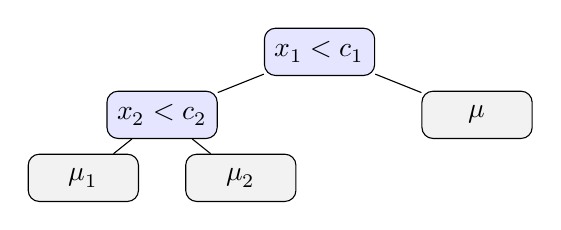
\begin{tikzpicture}[
						level 1/.style={level distance=8mm, sibling distance=40mm},
						level 2/.style={level distance=8mm, sibling distance=20mm},
						treenode/.style={rectangle, draw=black, rounded corners, minimum width=14mm, minimum height=6mm, align=center},
						internal/.style={treenode, fill=blue!10},
						term/.style={treenode, fill=gray!10}]
						\node[internal] {$x_1 < c_1$}
						child { node[internal] {$x_2 < c_2$}
							child { node[term] {$\mu_1$} }
							child { node[term] {$\mu_2$} }
						}
						child { node[term] {$\mu$} };
					\end{tikzpicture}
				};
			\end{scope}
		\end{tikzpicture}
		\caption{Full tree (left) and pruned tree (right).}
	\end{subfigure}
	
	\begin{subfigure}{\textwidth}
		\centering
		\begin{tikzpicture}[every node/.style={font=\footnotesize}]
			%----------------------------------
			% Arrow at origin
			%----------------------------------
			\node (arrow) at (0,0) {\Huge$\Longrightarrow$};
			
			%----------------------------------
			% Left tree (shifted left)
			%----------------------------------
			\begin{scope}[shift={(-3.5cm,0)}] % adjust based on left tree width
				\node {
					\begin{tikzpicture}[
						level 1/.style={level distance=8mm, sibling distance=40mm},
						level 2/.style={level distance=8mm, sibling distance=20mm},
						treenode/.style={rectangle, draw=black, rounded corners,
							minimum width=14mm, minimum height=6mm, align=center},
						internal/.style={treenode, fill=blue!10},
						term/.style={treenode, fill=gray!10}]
						\node[internal] {$x_3 < 0.5$}
						child { node[term] {$\mu_L$} }
						child { node[term] {$\mu_R$} };
					\end{tikzpicture}
				};
			\end{scope}
			
			%----------------------------------
			% Right tree (shifted right)
			%----------------------------------
			\begin{scope}[shift={(3.5cm,0)}] % adjust based on right tree width
				\node {
					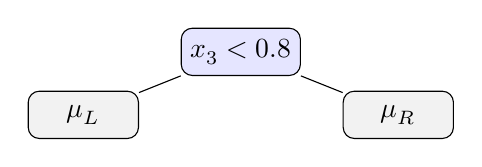
\begin{tikzpicture}[
						level 1/.style={level distance=8mm, sibling distance=40mm},
						level 2/.style={level distance=8mm, sibling distance=20mm},
						treenode/.style={rectangle, draw=black, rounded corners,
							minimum width=14mm, minimum height=6mm, align=center},
						internal/.style={treenode, fill=blue!10},
						term/.style={treenode, fill=gray!10}]
						\node[internal] {$x_3 < 0.8$}
						child { node[term] {$\mu_L$} }
						child { node[term] {$\mu_R$} };
					\end{tikzpicture}
				};
			\end{scope}
		\end{tikzpicture}
		\caption{Change of split threshold from $x_3 < 0.5$ to $x_3 < 0.8$.}
	\end{subfigure}
	
	\begin{subfigure}{\textwidth}
	
		\centering
		\begin{tikzpicture}[every node/.style={font=\footnotesize}]
			%----------------------------------
			% Arrow at origin
			%----------------------------------
			\node (arrow) at (0,0) {\Huge$\Longrightarrow$};
			
			%----------------------------------
			% Left tree (shifted left)
			%----------------------------------
			\begin{scope}[shift={(-4.5cm,0)}] % adjust -5cm based on left tree width
				\node {
					\begin{tikzpicture}[level 1/.style={level distance=8mm, sibling distance=40mm},
						level 2/.style={level distance=8mm, sibling distance=20mm},
						treenode/.style={rectangle, draw=black, rounded corners, minimum width=14mm, minimum height=6mm, align=center},
						internal/.style={treenode, fill=blue!10},
						term/.style={treenode, fill=gray!10}]
						\node[internal] {$x_1 < c_1$}
						child { node[internal] {$x_2 < c_2$}
							child { node[term] {$\mu_1$} }
							child { node[term] {$\mu_2$} }
						}
						child { node[term] {$\mu_3$} };
					\end{tikzpicture}
				};
			\end{scope}
			
			%----------------------------------
			% Right tree (shifted right)
			%----------------------------------
			\begin{scope}[shift={(4.5cm,0)}] % adjust 5cm based on right tree width
				\node {
					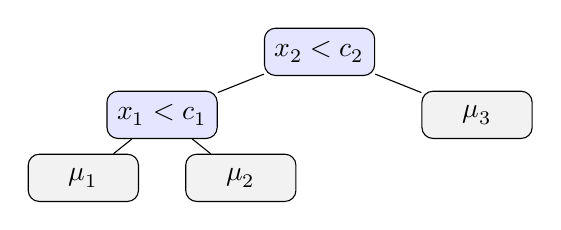
\begin{tikzpicture}[level 1/.style={level distance=8mm, sibling distance=40mm},
						level 2/.style={level distance=8mm, sibling distance=20mm},
						treenode/.style={rectangle, draw=black, rounded corners, minimum width=14mm, minimum height=6mm, align=center},
						internal/.style={treenode, fill=blue!10},
						term/.style={treenode, fill=gray!10}]
						\node[internal] {$x_2 < c_2$}
						child { node[internal] {$x_1 < c_1$}
							child { node[term] {$\mu_1$} }
							child { node[term] {$\mu_2$} }
						}
						child { node[term] {$\mu_3$} };
					\end{tikzpicture}
				};
			\end{scope}
		\end{tikzpicture}
		\caption{Original tree (left) and swapped version (right).}
	\end{subfigure}
	
	\caption{Graphical representation of tree MCMC moves}
	\label{fig:tree:MCMC}
\end{figure}


\subsection{Proposal for each moves}

Here, we explain the proposals of our RJ-MCMC algorithm for different tree moves. We follow the framework of \cite{green_RJMCMC} to define the acceptance probabilities corresponding to each move.


\subsubsection{\textsc{grow}/\textsc{prune} move:}
For growing a tree $T^{\ast}_k$ from $T_k$, we first randomly sample a terminal node $j$ from the set of all terminal nodes. Followed by a cut point for the splitting rule of the terminal node. Lastly, we sample terminal node values for the new left and right terminal nodes. Then we have the following:
\begin{equation*}
	q_{k;\gamma;\textsc{grow}}\left(T_k,M_k;T_k^{\ast}, M_k^{\ast}\right) 
	= \frac{1}{\#\{\mathcal{TN}(T_k)\}} \pi_{\textsc{rule}}(j\mid c)\mathcal{N}\left(\mu_{jr}^{\ast};\mu_{j},\gamma_{jr}\right)\mathcal{N}\left(\mu_{jl}^{\ast};\mu_{j},\gamma_{jl}\right),
\end{equation*} 
where $\mathcal{N}(a;b,c^2)$ is the probability of getting $a$ from a normal distribution with mean $b$ and variance $c^2$. Here $\mu_j$ is same for both the proposals as the value at observations remain same after growing. However, the variance contribution changes.

To go back from $T^{\ast}_k$ to $T_k$, we prune the $jl$-th terminal node and $jr$-th terminal node. For that, we calculate the probability of choosing the $j$-th node that becomes an internal node now. Followed by the proposal for terminal node value. Then,
\begin{equation*}
	q_{k;\gamma;\textsc{prune}}\left(T_k^{\ast}, M_k^{\ast};T_k,M_k\right) 
	= \frac{1}{\#\{\mathcal{PN}(T_k^{\ast})\}} \mathcal{N}\left(\mu_j;\mu^{\ast}_j,\gamma_j\right)
\end{equation*} 
where $\mu^{\ast}_j = \frac{ \#\{\mathcal{I}^k_{jr}\}\mu_{jr}^{\ast} +  \#\{\mathcal{I}^k_{jl}\}\mu_{jl}^{\ast}}{ \#\{\mathcal{I}^k_{jr}\}+ \#\{\mathcal{I}^k_{jl}\}}$. Therefore, the proposal ratio of the \textsc{growth} move is given by:
\begin{equation*}
	\frac{q_{k;\gamma;\textsc{prune}}\left(T_k^{\ast}, M_k^{\ast};T_k,M_k\right)}{q_{k;\gamma;\textsc{grow}}\left(T_k,M_k;T_k^{\ast}, M_k^{\ast}\right) } 
	= \frac{\frac{1}{\#\{\mathcal{PN}(T_k^{\ast})\}} \mathcal{N}\left(\mu_j;\mu_{j}^{\ast},\gamma_j\right)}{\frac{1}{\#\{\mathcal{TN}(T_k)\}} \pi_{\textsc{rule}}(j\mid c)\mathcal{N}\left(\mu_{jr}^{\ast};\mu_{j},\gamma_{jr}\right)\mathcal{N}\left(\mu_{jl}^{\ast};\mu_{j},\gamma_{jl}\right)}.
\end{equation*}
Similarly, we get the prior ratio for a \textsc{growth} move. Note that when a tree is grown at the $j$-th terminal node, we need additional splitting rule at that node. Therefore the ratio is given by:
\begin{equation*}
	\frac{\pi(T_k^{\ast},M_k^{\ast})\pi_{\textsc{rule}}(j\mid c)}{\pi(T_k,M_k)}.
\end{equation*}
Finally, combining with the likelihood we get
\begin{align*}
	&AR_{k;\gamma;\textsc{grow}}\left(T_k,M_k;T_k^{\ast}, M_k^{\ast}\right)\\
	&= \frac{
		\frac{\pi(T_k^{\ast},M_k^{\ast})}{\#\{\mathcal{PN}(T_k^{\ast})\}} 
		\prod_{i\in \mathcal{I}_{jr}^k}c\left(u_{1i},u_{2i}\mid h\left(R_{ik}+\mu^{\ast}_{jr}\right)\right)
		\prod_{i\in \mathcal{I}_{jl}^k}c\left(u_{1i},u_{2i}\mid h\left(R_{ik}+\mu^{\ast}_{jl}\right)\right)
		\mathcal{N}\left(\mu_j;\mu_{j}^{\ast},\gamma_j\right)}
	{\frac{\pi(T_k,M_k)}{\#\{\mathcal{TN}(T_k)\}} 
		\prod_{i\in \mathcal{I}_{j}^k}c\left(u_{1i},u_{2i}\mid h\left(R_{ik}+\mu_j\right)\right) 
		\mathcal{N}\left(\mu_{jr}^{\ast};\mu_{j},\gamma_{jr}\right)\mathcal{N}\left(\mu_{jl}^{\ast};\mu_{j},\gamma_{jl}\right)}.
\end{align*}
Since \textsc{prune} is the reverse process of the \textsc{grow} move, we have
\begin{align*}
	&AR_{k;\gamma;\textsc{prune}}\left(T_k,M_k;T_k^{\ast}, M_k^{\ast}\right)\\
	&= \frac{
		\frac{\pi(T^{\ast}_k,M^{\ast}_k)}{\#\{\mathcal{TN}(T^{\ast}_k)\}} 
		\prod_{i\in \mathcal{I}_{j}^k}c\left(u_{1i},u_{2i}\mid h\left(R_{ik}+\mu^{\ast}_j\right)\right) 
		\mathcal{N}\left(\mu_{jr};\mu^{\ast}_{j},\gamma_{jr}\right)
		\mathcal{N}\left(\mu_{jl};\mu^{\ast}_{j},\gamma_{jl}\right)}
	{\frac{\pi(T_k,M_k)}{\#\{\mathcal{PN}(T_k)\}} 
		\prod_{i\in \mathcal{I}_{jr}^k}c\left(u_{1i},u_{2i}\mid h\left(R_{ik}+\mu_{jr}\right)\right)
		\prod_{i\in \mathcal{I}_{jl}^k}c\left(u_{1i},u_{2i}\mid h\left(R_{ik}+\mu_{jl}\right)\right)
		\mathcal{N}\left(\mu^{\ast}_j;\mu_{j},\gamma_j\right)}
\end{align*}
where $\mu_j = \frac{\#\{\mathcal{I}^k_{jr}\}\mu_{jr} + \#\{\mathcal{I}^k_{jl}\}\mu_{jl}}{\#\{\mathcal{I}^k_{jr}\} + \#\{\mathcal{I}^k_{jl}\}}$.

\subsubsection{\textsc{change}/\textsc{swap} move:}
For the \textsc{change} or the \text{swap} move. The proposals only rely on the internal nodes and the terminal nodes and values remain unchanged. Moreover, for each of these moves $\mathcal{IN}(T_k)$ and $\mathcal{PCN}(T_k)$ remain invariant in nature. That is for a proposed tree $T_k^{\ast}$, $\mathcal{IN}(T_k)=\mathcal{IN}(T_k^{\ast})$ and $\mathcal{PCN}(T_k)=\mathcal{PCN}(T_k^{\ast})$. Therefore, the proposal ratios of these two moves are equal to 1. This gives the following:

\begin{align*}
	AR_{k;\gamma;\textsc{move}}\left(T_k,M_k;T_k^{\ast}, M_k^{\ast}\right)= \frac{
		\pi(T^{\ast}_k,M^{\ast}_k) 
		\prod_{i=1}^{n}c\left(u_{1i},u_{2i}\mid h\left(R_{ik}+g(x_i, T_k^{\ast}, M_k^{\ast})\right)\right)}
	{\pi(T_k,M_k) 
		\prod_{i=1}^{n}c\left(u_{1i},u_{2i}\mid h\left(R_{ik}+g(x_i, T_k, M_k)\right)\right)}
\end{align*}
for $\textsc{move}\in\{\textsc{change},\textsc{swap}\}$.

Once we have the acceptance ratio, we can calculate the acceptance probability $\alpha_{k;\gamma;\textsc{move}}\left(T_k,M_k;T_k^{\ast}, M_k^{\ast}\right)$ of moving from $(T_k,M_k)$ to $(T_k^{\ast},M_k^{\ast})$ in the following way:
\begin{equation*}
	\alpha_{k;\gamma;\textsc{move}}\left(T_k,M_k;T_k^{\ast}, M_k^{\ast}\right) = \min\left\{1,AR_{k;\gamma;\textsc{move}}\left(T_k,M_k;T_k^{\ast}, M_k^{\ast}\right)\right\},
\end{equation*}
where $\textsc{move}\in \left\{\textsc{grow}, \textsc{prune}, \textsc{change}, \textsc{swap}\right\}$.


\subsection{Markov transition kernel of the RJ-MCMC step}

Let $\mathcal{S}\coloneqq\mathcal{T}\times \mathcal{M}$ be the state space and $S_k\coloneqq(T_k,M_k) \in \mathcal{S}$ be the current state of the $k$-th tree. Let $p_{\textsc{g}}$, $p_{\textsc{p}}$, $p_{\textsc{c}}$ and $p_{\textsc{s}}$ be the probabilities of selecting \textsc{grow}, \textsc{prune}, \textsc{change} and \textsc{swap} move respectively. Then dropping the tree index $k$ for convenience, we can write the transition kernel of the RJ-MCMC algorithm with $\gamma$ adaption in the following way:
\begin{align*}
	\mathcal{K}_{\gamma}\left(s; \cdot\right) 
	= p_{\textsc{g}}\mathcal{K}_{\gamma;\textsc{grow}}\left(s; \cdot\right) + 
	p_{\textsc{p}}\mathcal{K}_{\gamma;\textsc{prune}}\left(s; \cdot\right) + 
	p_{\textsc{c}}\mathcal{K}_{\gamma;\textsc{change}}\left(s; \cdot\right)+ 
	p_{\textsc{s}}\mathcal{K}_{\gamma;\textsc{swap}}\left(s; \cdot\right).
\end{align*}
Here, for the \textsc{change} and \textsc{swap} moves, we do not need to propose any new terminal node values hence $\gamma$ adaption is not utilised and the notation is used for the sake of consistency. Now, let $s^{\ast}$ be a proposed state, then each of these kernels with $\gamma$ adaption are given by
\begin{align*}
	\mathcal{K}_{\gamma;\textsc{move}}\left(s, \cdot\right) 
	&= \alpha_{\gamma;\textsc{move}}\left(s;s^{\ast}\right) 
	q_{\gamma;\textsc{move}}\left(s;s^{\ast}\right)ds^{\ast} \\
	&\qquad+ \left(1 - \int_{\mathcal{T}\times\mathcal{M}} \alpha_{\gamma;\textsc{move}}\left(s;s^{\ast}\right) 
	q_{\gamma;\textsc{move}}\left(s;s^{\ast}\right)ds^{\ast}\right) \delta_{s}(ds^{\ast}),
\end{align*}
where $\textsc{move}\in \left\{\textsc{grow}, \textsc{prune}, \textsc{change}, \textsc{swap}\right\}$ and $\delta_x(dy)$ is the Dirac measure at $x$. 

\subsubsection{Adaptive proposal variance} 

For the sake of notational consistency, we restate the algorithm for computing the adaptive proposal variance in \cref{alg:ada:prop} without the tree index.

\begin{algorithm}[h]
	\caption{Computation of adaptive proposal}\label{alg:ada:prop}
	\begin{algorithmic}[1]
		\State Perform $\eta_0$ iterations with a fixed variance.
		
		\State Collect MCMC samples for initial $\eta_0$ iterations:
		\begin{equation*}
			V_{i}^{\eta} = g\left(x_i,T^{\eta},M^{\eta}\right)\quad 1\le i \le n; 1\le \eta \le \eta_0.
		\end{equation*}
		
		\State Calculate sample covariance matrix :
		\begin{equation*}
			C^{\eta} \coloneqq Cov\left(V^{1},V^{2},\cdots,V^{\eta}\right) + \epsilon\mathbf{I}_n \quad \text{for } \epsilon>0; \eta>\eta_0.
		\end{equation*}
		
		\State Calculate the proposal variance of the $j$-th terminal node value:
		\begin{equation*}
			\sigma_{\text{prop};j}^2 \coloneqq \frac{2.4^2}{\left(\#\left\{\mathcal{I}_{j}\right\}\right)^3}
			\sum_{c\in\mathcal{I}_{j}}\sum_{d\in\mathcal{I}_{j}}\left[C^{\eta}\right]_{cd};\qquad\mathcal{I}_{j}\coloneqq \left\{i:x_i\in \Omega_{j}\right\};\qquad 1\le j\le n_L(T).
		\end{equation*}
		
		\State Update sample covariance using 
		\begin{equation*}
			C^{\eta+1} \coloneqq 
			\frac{\eta-1}{\eta} C^{\eta} 
			+ \frac{1}{\eta}\left(\eta 
			\left(\overline{V}^{\eta}\right)\left(\overline{V}^{\eta}\right)^T 
			- (\eta+1)\left(\overline{V}^{\eta+1}\right)\left(\overline{V}^{\eta+1}\right)^T 
			+ \left({V}^{\eta+1}\right)\left({V}^{\eta+1}\right)^T + \epsilon\mathbf{I}_n\right).
		\end{equation*}
	\end{algorithmic}
\end{algorithm}



\subsection{Proof of Ergodicity}

Before providing the proof of ergodicity. We restate the required assumptions and prove two lemmas that are necessary for showing ergodicity.

\begin{assumption}\label{ass:bounded:cop}
	$\exists$ \(\delta>0\) such that the copula density is bounded. That is, $0 < c(u_1,u_2\mid\theta(h(g(x,T,M)))) < \infty$ for all $(u_1,u_2)\in[\delta,1-\delta]^2$ and for all $M \in \mathcal{M}$
\end{assumption}
\begin{assumption}\label{ass:bounded:prior}
	All prior densities for the terminal node values are bounded above.
\end{assumption}
\begin{assumption}\label{ass:bounded:prop}
	All proposal densities of the terminal node values are uniformly bounded.
\end{assumption}
\begin{assumption}\label{ass:bounded:tree}
	With $n$ observations, the number of terminal nodes $n_L(T)\le n$ and for any tree with $n_L(T)\ge 2$, there exists at least one internal node that can be pruned.
\end{assumption}


Now, let $S\coloneqq \left(T,M\right)$ be a state in the state space $\mathcal{S}\coloneqq\mathcal{T}\times \mathcal{M}$. Let $\Gamma^{\eta} \coloneqq \left(\Gamma_{1}^{\eta}, \cdots\Gamma^{\eta}_{n_L(T)}\right)\in\mathcal{Y}$ be the adaption at the $\eta$-th iteration such that for $j \in \{1,2,\cdots, n_L(T)\}$
\begin{equation*}
	\Gamma^{\eta}_{j} \coloneqq \frac{2.4^2}{\left(\#\left\{\mathcal{I}_{j}\right\}\right)^3}
	\sum_{c\in\mathcal{I}_{j}}\sum_{d\in\mathcal{I}_{j}}\left[C^{\eta}\right]_{cd}.
\end{equation*}
Then the following two lemmas are true.

\begin{lemma}\label{lemm:bounded:ratio}
	If \cref{ass:bounded:cop}-\cref{ass:bounded:prop} are satisfied then the acceptance ratios are uniformly bounded. That is, there exist values $0< b_{\textsc{move}} <  B_{\textsc{move}} < \infty$ such that
	\begin{equation*}
		\frac{1}{B_{\textsc{move}}} \le AR_{\gamma, \textsc{move}}\left(s;s^{\ast}\right) \le \frac{1}{b_{\textsc{move}}}
	\end{equation*}
	$\forall\gamma \in \mathcal{Y}$.
\end{lemma}

\begin{proof}
	In a compact support of $[\delta,1-\delta]^2$, the bivariate copula density functions presented in this article are bounded. Besides this, the prior and proposal for a tree is from a discrete space and the priors and proposals for the terminal node values have finite variances. Therefore, the posterior is bounded for all possible terminal node values in $\mathcal{M}$. Moreover, since the proposal variances are uniformly bounded \citep{haario_AMH}, the bounds of the acceptance ratios are independent of the $\gamma$ adaption.
\end{proof}

This lemma ensures that we do not have degenerate values for the acceptance rate which is otherwise problematic for the convergence of MCMC algorithm.

\begin{lemma}\label{lemm:stable:var}
	$\left\|\Gamma^{\eta+1}_{j} - \Gamma^{\eta}_{j}\right\|_{\infty}\to 0$ as $\eta\to\infty$.
\end{lemma}

\begin{proof}
	Recall the iterative variance formula given by:
	\begin{equation*}
		C^{\eta+1} \coloneqq 
		\frac{\eta-1}{\eta} C^{\eta} 
		+ \frac{1}{\eta}\left(\eta 
		\left(\overline{V}^{\eta}\right)\left(\overline{V}^{\eta}\right)^T 
		- (\eta+1)\left(\overline{V}^{\eta+1}\right)\left(\overline{V}^{\eta+1}\right)^T 
		+ \left({V}^{\eta+1}\right)\left({V}^{\eta+1}\right)^T + \epsilon\mathbf{I}_n\right),
	\end{equation*}
	where $\overline{V}^{\eta}$ is the point-wise mean of $\eta$ MCMC samples. That is, for $n$ number of observations $\overline{V}^{\eta} \coloneqq \left(\frac{1}{\eta}\sum_{i=1}^\eta V_1^i,\cdots, \frac{1}{\eta}\sum_{i=1}^\eta V_n^i\right)^T$. Using this iterative formula, we define the change in variance in two consecutive iterations in the following way:
	\begin{equation*}
		\Delta C^{\eta + 1} \coloneqq \frac{1}{\eta}\left(\eta \left(\overline{V}_{\cdot }^{\eta}\right)\left(\overline{V}_{\cdot }^{\eta}\right)^T 
		- (\eta+1)\left(\overline{V}_{\cdot }^{\eta+1}\right)\left(\overline{V}_{\cdot }^{\eta+1}\right)^T 
		+ \left({V}_{\cdot }^{\eta+1}\right)\left({V}_{\cdot }^{\eta+1}\right)^T + \epsilon\mathbf{I}_n - C^{\eta}\right).
	\end{equation*}
	Now, let $ n_j = \#\left\{\mathcal{I}_{j}\right\}$ denote the number of observations contained in the $j$-th partition. Then
	\begin{align*}
		\Gamma^{\eta+1}_j 
		= \frac{2.4^2}{\left(n_{j}\right)^3}
		\sum_{c\in\mathcal{I}_{j}}\sum_{d\in\mathcal{I}_{j}}\left[C^{\eta+1}\right]_{cd}
		&= \frac{2.4^2}{\left(n_{j}\right)^3}
		\left[\sum_{c\in\mathcal{I}_{j}}\sum_{d\in\mathcal{I}_{j}}\left[C^{\eta} + \Delta C^{\eta + 1}\right]_{cd}\right] \\
		&= \Gamma^{\eta}_j + \frac{2.4^2}{\left(n_{j}\right)^3} \left[\sum_{c\in\mathcal{I}_{j}}\sum_{d\in\mathcal{I}_{j}}\left[\Delta C^{\eta + 1}\right]_{cd}\right].
	\end{align*}
	Since $\overline{V}^{\eta} \coloneqq \left(\frac{1}{\eta}\sum_{i=1}^\eta V_1^i,\cdots, \frac{1}{\eta}\sum_{i=1}^\eta V_n^i\right)^T$ and $\overline{V}^{\eta+1} \coloneqq \left(\frac{1}{\eta+1}\sum_{i=1}^{\eta+1} V_1^i,\cdots, \frac{1}{\eta+1}\sum_{i=1}^{\eta+1} V_n^i\right)^T$, the increment is of $O(1/\eta)$ in the $(\eta +1)$-th iteration. Therefore $\left\|\Gamma^{\eta+1}_j - \Gamma^{\eta}_j\right\|_{\infty} \to 0$ as $\eta\to \infty$.
\end{proof}
This way, we ensure that variance in each iterative steps does not change rapidly and eventually the change becomes infinitesimally small.

\begin{manualtheorem}{4.1}
	If \cref{ass:bounded:cop}-\cref{ass:bounded:tree} are satisfied and $\gamma$ adaption strategy is defined by \cref{alg:ada:prop}. Then the following two conditions hold:
	\begin{enumerate}
		\item Diminishing adaptation $\rightarrow$ $\left\|\mathcal{K}_{\Gamma^{\eta+1}}(s;\cdot)-\mathcal{K}_{\Gamma^{\eta}}(s;\cdot)\right\|_{TV}\to 0$ in probability as $\eta\to \infty$.
		\item Containment $\rightarrow$ $\forall\iota>0$, $\exists N = N(\iota)\in \mathbb{N}$ such that 
		\begin{equation*}
			\left\|\mathcal{K}^N_{\gamma}(s;\cdot) - \pi(\cdot\mid u_1,u_2)\right\|_{TV} \le \iota
		\end{equation*}
	\end{enumerate}
	where $\pi(\cdot\mid u_1, u_2)$ denote the target distribution defined on $\mathcal{S}$.
\end{manualtheorem}

\begin{proof}
	\textbf{Diminishing adaptation:}
	To show diminishing adaptation, we check the total variation norm for each move. Let the \textsc{grow} move is denoted by \textsc{g}. Then the kernel corresponding \textsc{grow} gives us
	\begin{align*}
		&\left\|\mathcal{K}_{\Gamma^{\eta+1};\textsc{g}}(s;\cdot)-\mathcal{K}_{\Gamma^{\eta};\textsc{g}}(s;\cdot)\right\|_{TV}\\
		&\le 2\int \left|\alpha_{\Gamma^{\eta+1};\textsc{g}}(s;s^{\ast})q_{\Gamma^{\eta+1};\textsc{g}}(s;s^{\ast}) - \alpha_{\Gamma^{\eta};\textsc{g}}(s;s^{\ast})q_{\Gamma^{\eta};\textsc{g}}(s;s^{\ast})\right|ds^{\ast}\\
		&\le 2\int \left|\alpha_{\Gamma^{\eta+1};\textsc{g}}(s;s^{\ast})\left(q_{\Gamma^{\eta+1};\textsc{g}}(s;s^{\ast}) - q_{\Gamma^{\eta};\textsc{g}}(s;s^{\ast})\right)\right|ds^{\ast} 
		+ 2\int \left|\left(\alpha_{\Gamma^{\eta+1};\textsc{g}}(s;s^{\ast})-\alpha_{\Gamma^{\eta};\textsc{g}}(s;s^{\ast})\right)q_{\Gamma^{\eta};\textsc{g}}(s;s^{\ast})\right|ds^{\ast}\\
		&\le 2\int \left|q_{\Gamma^{\eta+1};\textsc{g}}(s;s^{\ast}) - q_{\Gamma^{\eta};\textsc{g}}(s;s^{\ast})\right|ds^{\ast} 
		+ 2\int \left|\left(\alpha_{\Gamma^{\eta+1};\textsc{g}}(s;s^{\ast})-\alpha_{\Gamma^{\eta};\textsc{g}}(s;s^{\ast})\right)q_{\Gamma^{\eta};\textsc{g}}(s;s^{\ast})\right|ds^{\ast}.
	\end{align*}
	
	Since $q_{\Gamma^{\eta+1};\textsc{g}}(s;s^{\ast})$ is a product of Gaussian probabilities with bounded variances and the adaption $\Gamma^{\eta+1}$ converges to $\Gamma^{\eta}$ by \cref{lemm:stable:var}, we can show that $\left\|q_{\Gamma^{\eta+1};\textsc{g}}(s;s^{\ast})-q_{\Gamma^{\eta};\textsc{g}}(s;s^{\ast})\right\|_{TV}$ goes to 0 as $\eta \to \infty$. Similarly, from \cref{lemm:bounded:ratio}, we know that the acceptance ratio and the proposal are uniformly bounded and the sequence $\alpha_{\gamma;\textsc{g}}(s;s^{\ast})$ is trivially dominated by 1. Hence exploiting the pointwise convergence of $\Gamma^{\eta}$ and continuity of $\alpha_{\Gamma^{\eta+1}}(s;s^{\ast})$, we can apply dominated convergence theorem and show that $\left\|\left(\alpha_{\Gamma^{\eta+1};\textsc{g}}(s;s^{\ast})-\alpha_{\Gamma^{\eta};\textsc{g}}(s;s^{\ast})\right)q_{\Gamma^{\eta};\textsc{g}}(s;s^{\ast})\right\|_{TV}$ goes to 0 as $\eta \to \infty$. Hence $\left\|\mathcal{K}_{\Gamma^{\eta+1};\textsc{g}}(s;\cdot)-\mathcal{K}_{\Gamma^{\eta};\textsc{g}}(s;\cdot)\right\|_{TV}$ goes to 0 as $\eta\to \infty$.
	
	With a similar argument for the \textsc{prune} move, we have $\left\|\mathcal{K}_{\Gamma^{\eta+1};\textsc{p}}(s;\cdot)-\mathcal{K}_{\Gamma^{\eta};\textsc{p}}(s;\cdot)\right\|_{TV}$ goes to 0 as $\eta\to \infty$. For \textsc{change} and \textsc{swap} moves, no adaption takes place. Therefore, we can show that the diminishing adaption holds for our proposed adaptive RJ-MCMC algorithm.
	
	\textbf{Containment:}
	To show the containment condition, we follow a similar approach to that of \citet{andrieu_RJ_MCMC}. Recall the state space denoted by $\mathcal{S}\coloneqq\mathcal{T}\times\mathcal{M}$. Then by \cref{ass:bounded:tree}, we can express this space as a finite union of subspaces such that $\mathcal{S} \coloneq \bigcup_{i=1}^n \mathcal{S}_i$, where $\mathcal{S}_i = \mathcal{T}_i \times \mathcal{M}_i$ is the space of all trees with $i$ terminal nodes and the corresponding vector of terminal nodes of length $i$ and $\mathcal{M}_i\subseteq\mathbb{R}^i$. 
	
	We will show that the Markov transition kernel $\mathcal{K}_{\gamma}(\cdot;\cdot)$ satisfies the minorisation condition \citep{meyn_tweedie1994} on the state space $\mathcal{S}$. That is the state space is a small set. First, we show that from any tree with $i$ terminal nodes, we can explore other trees with non zero probability.
	
	Let $s_i \coloneqq\left(T^{(i)}, M^{(i)}\right)$ denote a pair of tree with $i$ terminal nodes and corresponding vector of terminal node values. Then for each $i=2,\cdots,n$, and $B_{i-1}\subseteq \mathcal{S}_{i-1}$
	\begin{align*}
		\mathcal{K}_{\gamma}\left(s_i;B_{i-1}\right)
		&\ge p_{\textsc{p}}\int_{B_{i-1}}\mathcal{K}_{\gamma,\textsc{prune}}\left(s_i;ds_{i-1}\right)\\
		&\ge p_{\textsc{p}}\int_{B_{i-1}}\alpha_{\gamma;\textsc{prune}}\left(s_i;s_{i-1}\right)q_{\gamma;\textsc{prune}}\left(s_i;s_{i-1}\right)ds_{i-1}\\
		&\ge \frac{p_{\textsc{p}}}{B_{\textsc{prune}}}\int_{B_{i-1}}q_{\gamma;\textsc{prune}}\left(s_i;s_{i-1}\right)ds_{i-1}.
	\end{align*}
	Therefore there exist a uniform lower bound $\nu>0$ independent of $\gamma$ such that for all $i=2,\cdots,n$ and $\gamma\in \mathcal{Y}$ the following holds
	\begin{equation}\label{eq:reach:trivial}
		\mathcal{K}_{\gamma}\left(s_i;B_{i-1}\right)
		\ge \nu\int_{B_{i-1}}q_{\gamma;\textsc{prune}}\left(s_i;s_{i-1}\right)ds_{i-1}.
	\end{equation}
	
	Now, let $s_1 = \left(T^{(1)},M^{(1)}\right)$ denote the trivial tree. That is, a tree with only one node. Then for all $i=2,\cdots, n$, we can reach the trivial tree with non-zero probability. Hence, we can define a measure $\phi$ such that
	\begin{equation*}
		\phi(A) = \int_{\mathcal{M}_1}\mathbb{I}\left(s_1\in A\right)\mathcal{N}\left(\mu;0,\sigma_1^2\right)d\mu
	\end{equation*}
	where $\sigma^2_1$ is the prior variance for terminal node value of the trivial tree. We will use this measure to satisfy the minorisation condition. Moreover, we can use this measure to show that $\mathcal{K}_{\gamma}(\cdot;\cdot)$ is $\phi$-irreducible. 
	
	Aperiodicity of the $\mathcal{K}_{\gamma}(\cdot;\cdot)$ is also achieved through construction. For instance, we can propose $s_2$ for which $\alpha_{\gamma;\textsc{grow}}\left(s_1; s_1\right) < 1$, independent of $\gamma$. Then the rejection probability $r_{\gamma;\textsc{grow}}\left(s_1\right)$ is given by:
	\begin{align*}
		r_{\gamma;\textsc{grow}}\left(s_1\right)
		&=1-\int \alpha_{\gamma;\textsc{grow}}\left(s_1; s_2\right)q_{\gamma;\textsc{grow}}\left(s_1; s_2\right) ds_2\\
		&=\int\left(1 - \alpha_{\gamma;\textsc{grow}}\left(s_1; s_2\right)\right) q_{\gamma;\textsc{grow}}\left(s_1; s_2\right) ds_2 > 0.
	\end{align*}
	Therefore, $\forall\gamma\in\mathcal{Y}$, there exists $1>\nu_0 >0$ such that
	\begin{equation}\label{eq:stay:trivial}
		\mathcal{K}_{\gamma}\left(s_1;\left\{s_1\right\}\right) \ge \nu_0 = \nu_0 \phi\left(\left\{s_1\right\}\right).
	\end{equation}
	
	Now, to show that minorisation holds on $\mathcal{S}$, we iterate the transition kernel $n$ times and using Chapman Kolmogorov equation we get
	\begin{align*}
		\mathcal{K}_{\gamma}^n\left(s_k;s_1\right)
		= \int_{\mathcal{S}}\mathcal{K}_{\gamma}^{k-1}\left(s_k;s\right)\mathcal{K}_{\gamma}^{n+1-k}\left(s;s_1\right)ds
		& \ge \int_{\mathcal{S}_1}\mathcal{K}_{\gamma}^{k-1}\left(s_k;s\right)\mathcal{K}_{\gamma}^{n+1-k}\left(s;s_1\right)ds\\
		& = \mathcal{K}_{\gamma}^{k-1}\left(s_k;s_1\right)\mathcal{K}_{\gamma}^{n+1-k}\left(s_1;\left\{s_1\right\}\right).
	\end{align*}
	Therefore, from \cref{eq:reach:trivial} and \cref{eq:stay:trivial}, we get 
	\begin{equation*}
		\mathcal{K}_{\gamma}^n\left(s_k;s_1\right) \ge \nu^{k-1} \nu_0^{n+1-k}\phi\left(s_1\right).
	\end{equation*}
	This holds true for $k=1$ as well. Therefore, for any $s_{k'}$ in $\mathcal{S}$,  
	\begin{equation*}
		\mathcal{K}_{\gamma}^n\left(s_k;s_{k'}\right) \ge \vartheta\phi\left(s_{k'}\right)
	\end{equation*}
	where $\vartheta = \min_{1\le k\le n}\left\{\nu^{k-1} \nu_0^{n+1-k}\right\}$. This shows that the state space $\mathcal{S}$ is small \citep{meyn_tweedie1994}. Then following the proposition given by \citet{Tierney1994}, we can find a constant $L_0>0$ such that for all $N$
	\begin{equation}
		\left\|\mathcal{K}^N_{\gamma}(s;\cdot) - \pi(\cdot\mid y)\right\|_{TV} \le L_0 (1-\vartheta)^{\lfloor N/n\rfloor}.
	\end{equation}
	Therefore, $K_{\gamma}(s;)$ is uniformly ergodic for all values of $\gamma$ and $s$. Hence, for all $\iota>0$, we can find $N = n\left(\frac{\log(\iota)-\log(L_0)}{\log(1-\vartheta)} +1\right)$ such that
	\begin{equation}
		\left\|\mathcal{K}^N_{\gamma}(s;\cdot) - \pi(\cdot\mid y)\right\|_{TV} \le \iota \qquad\forall s\in \mathcal{S}, \gamma\in\mathcal{Y}.
	\end{equation}
	
\end{proof}

\section{Synthetic dataset}\label{app:results}

\subsection{Tree structure datasets}
We present the traceplots of the number of terminal nodes in \cref{fig:trace:nterm:ex1} and the depth in \cref{fig:trace:depth:ex1} for the first replicate corresponding to each copula. We notice that the tree exploration stabilises after about 1000 iterations with our proposed approaches. We also present the likelihood plot after discarding 1500 burn in samples in \cref{fig:trace:like:ex1}. We see that our method is able to converge towards the true likelihood region for all cases, shown by the black dashed line. 

\begin{figure}
	\centering
	\includegraphics[width = 0.8\linewidth]{"case_1_nterm.pdf"}
	\caption{Trace plots of the number of terminal nodes obtained from our analyses with synthetic datasets generated using tree based Kendall's tau, for the first replicate. The plots are obtained by running 4 parallel chains, each one with 3000 MCMC iterations. The left column shows analyses with C-BART and the right column shows analyses with A-C-BART. The horizontal dashed black line represents the number of terminal nodes (3) of the data-generating tree.}
	\label{fig:trace:nterm:ex1}
\end{figure}

\begin{figure}
	\centering
	\includegraphics[width = 0.8\linewidth]{"case_1_depth.pdf"}
	\caption{Trace plots of the depth of the tree obtained from our analyses with synthetic datasets generated using tree based Kendall's tau, for the first replicate. The plots are obtained by running 4 parallel chains, each one with 3000 MCMC iterations. The left column shows analyses with C-BART and the right column shows analyses with A-C-BART. The horizontal dashed black line represents the depth (2) of the data-generating tree.}
	\label{fig:trace:depth:ex1}
\end{figure}

\begin{figure}
	\centering
	\includegraphics[width = 0.8\linewidth]{"case_1_likelihood.pdf"}
	\caption{Trace plots of the log-likelihood obtained from our analyses with synthetic datasets generated using tree based Kendall's tau, for the first replicate. The plots are obtained by running 4 parallel chains, each one with 3000 MCMC iterations. The left column shows analyses with C-BART and the right column shows analyses with A-C-BART. The horizontal dashed black line represents the true log-likelihood of the data-generating tree.}
	\label{fig:trace:like:ex1}
\end{figure}

We present the traceplots of the number of terminal nodes, depth and likelihood for the Frank copula in \cref{fig:trace:frank} when the proposal variance is 0.2. We notice that for the first dataset, only one out of 4 chains converge to true likelihood region for C-BART after 7500 iterations, whereas all 4 chains converge to the true likelihood region for A-C-BART. We also present the efficiency of our methods in finding the true tree structure in \cref{tab:eff:ex1:frank} and prediction accuracy in \cref{tab:pred:ex1:frank}.

\begin{figure}[H]
	\centering
	\includegraphics[width = 0.85\linewidth]{"frank_longer_sim.pdf"}
	\caption{Trace plots of the likelihood; the number of terminal nodes; and the depth of the tree for the first replicate of the Frank copula datasets generated using tree based Kendall's tau. The plots are obtained by running 4 parallel chains with 7500 MCMC iterations each and proposal variance fixed at $0.2$. The left column shows analyses with C-BART and the right column shows analyses with A-C-BART.}
	\label{fig:trace:frank}
\end{figure}

\begin{table}[H]
	\centering
	\begin{tabular}{l|cccccc}
		& Mean ($\hat{n}_L$) & SD ($\hat{n}_L$) & Mean ($\hat{D}$) & SD ($\hat{D}$) & Mean Acc. & SD Acc. \\ 
		\midrule
		Frank (C-BART) & 2.242 & 0.277 & 1.232 & 0.265 & 0.111 & 0.029 \\
		Frank (A-C-BART) & 2.592 & 0.343 & 1.569 & 0.329 & 0.117 & 0.024 \\
	\end{tabular}
	\caption{Performance of our proposed method for Frank copula dataset using a tree based conditional Kendall's tau. We present the average and the standard deviation of the posterior expectation of the number of terminal nodes and the depth of the tree along with the acceptance rate. The quantities are obtained by running 4 parallel chains with 7500 MCMC iterations each and proposal variance fixed at $0.2$.}
	\label{tab:eff:ex1:frank}
\end{table}

\begin{table}[H]
	\centering
	\begin{tabular}{l|ccc|ccc}
		\multicolumn{1}{c|}{} &
		\multicolumn{3}{c|}{C-BART} &
		\multicolumn{3}{c}{A-C-BART} \\
		\midrule
		& RMSE & CI-length & CI-cov & RMSE & CI-length & CI-cov \\ 
		\midrule
		Frank & 0.194 & 0.224 & 0.432 & 0.153 & 0.244 & 0.688 
	\end{tabular}
	\caption{Prediction accuracy of our proposed method for the Frank copula datasets using a tree based conditional Kendall's tau. We split our results in two general columns: left for C-BART, right for A-C-BART. We create subcolumns under each column to present root mean squared error (RMSE); average 95\% credible interval length (CI-length); and 95\% credible interval coverage (CI-cov). The quantities are obtained by running 4 parallel chains with 7500 MCMC iterations each and proposal variance fixed at $0.2$.}
	\label{tab:pred:ex1:frank}
\end{table}

\subsection{Dataset with a general function}

We present the prediction plots corresponding to the first replicate of the copula datasets in \cref{fig:trace:pred:ex2}. In the figure, we represent the true values of Kendall's conditional tau with red points; posterior estimates of Kendall's tau with a black line and credible intervals with green lines. 

Additionally, we present the likelihood traceplots in \cref{fig:trace:like:ex2}. We notice that both C-BART and A-C-BART are able to move towards the true likelihood region, suggesting the efficiency of our method in exploring the parameter space.

\begin{figure}
	\centering
	\includegraphics[width = 0.8\linewidth]{"case_2_pred.pdf"}
	\caption{Comparison of BART fit obtained from our analyses with synthetic datasets generated using a non-linear Kendall's tau, for the first replicate. The plots are obtained by running 4 parallel chains, each one with 3000 MCMC iterations. The left column shows analyses with C-BART and the right column shows analyses with A-C-BART. The green lines denote the 95\% credible interval; the black line denotes the posterior estimate of Kendall's tau; and the red points show the true values of conditional Kendall's tau.}
	\label{fig:trace:pred:ex2}
\end{figure}

\begin{figure}
	\centering
	\includegraphics[width = 0.8\linewidth]{"case_2_likelihood.pdf"}
	\caption{Trace plots of the log-likelihood obtained from our analyses with synthetic datasets generated using a non-linear Kendall's tau, for the first replicate. The plots are obtained by running 4 parallel chains, each one with 3000 MCMC iterations. The left column shows analyses with C-BART and the right column shows analyses with A-C-BART. The horizontal dashed black line represents the true log-likelihood of the data-generating tree.}
	\label{fig:trace:like:ex2}
\end{figure}

\section{CIA world fact data}\label{app:cia}
Additional figures for simulated copulas
\begin{figure}
	\centering
	\includegraphics[width = 0.95\linewidth]{"LE_vs_GDP_woa.pdf"}
	\caption{Scatter plots of pseudo observations and simulated values from the fitted copulas obtained for life expectancy of male and female populations using C-BART with 5 trees.}
	\label{fig:pseudo:LE:woa}
\end{figure}
\begin{figure}
	\centering
	\includegraphics[width = 0.95\linewidth]{"LE_vs_GDP_wa.pdf"}
	\caption{Scatter plots of pseudo observations and simulated values from the fitted copulas obtained for life expectancy of male and female populations using A-C-BART with 5 trees.}
	\label{fig:pseudo:LE:wa}
\end{figure}

\begin{figure}
	\centering
	\includegraphics[width = 0.95\linewidth]{"LT_vs_GDP_woa.pdf"}
	\caption{Scatter plots of pseudo observations and simulated values from the fitted copulas obtained for literacy of male and female population using C-BART with 5 trees.}
	\label{fig:pseudo:LT:woa}
\end{figure}
\begin{figure}
	\centering
	\includegraphics[width = 0.95\linewidth]{"LT_vs_GDP_wa.pdf"}
	\caption{Scatter plots of pseudo observations and simulated values from the fitted copulas obtained for literacy of male and female population using A-C-BART with 5 trees.}
	\label{fig:pseudo:LT:wa}
\end{figure}



Additional figures related to our analyses with 10 trees.
\begin{figure}[H]
	\centering
	\includegraphics[width = 0.75\linewidth]{"LE_vs_GDP_taus_10.pdf"}
	\caption{Estimated dependence between male life expectancy and female life expectancy conditional on log-GDP. For modelling, we use 10 trees and run 4 parallel chains of 50000 iterations. For posterior inference, we discard the first 5000 samples.}
	\label{fig:taus:LE10}
\end{figure}

\begin{figure}[H]
	\centering
	\includegraphics[width = 0.75\linewidth]{"LE_vs_GDP_likelihood_10.pdf"}
	\caption{Trace plots of the log-likelihood obtained from our analyses with life expectancies of the male and female populations. The plots are obtained by running 4 parallel chains, each with 50000 MCMC iterations and 10 trees. The left columns shows analyses with C-BART and the right column shows analyses with A-C-BART.}
	\label{fig:trace:like:real:LE10}
\end{figure}

\begin{figure}[H]
	\centering
	\includegraphics[width = 0.75\linewidth]{"LE_vs_GDP_woa_10.pdf"}
	\caption{Scatter plots of pseudo observations and simulated values from the fitted copulas obtained for life expectancy of male and female population using C-BART with 10 trees.}
	\label{fig:pseudo:LE:woa10}
\end{figure}

\begin{figure}[H]
	\centering
	\includegraphics[width = 0.75\linewidth]{"LE_vs_GDP_wa_10.pdf"}
	\caption{Scatter plots of pseudo observations and simulated values from the fitted copulas obtained for life expectancy of male and female population using A-C-BART with 10 trees.}
	\label{fig:pseudo:LE:wa10}
\end{figure}

\begin{figure}[H]
	\centering
	\includegraphics[width = 0.75\linewidth]{"LT_vs_GDP_likelihood_10.pdf"}
	\caption{Trace plots of the log-likelihood obtained from our analyses with literacy rates of the male and female populations. The plots are obtained by running 4 parallel chains, each with 50000 MCMC iterations and 10 trees. The left columns shows analyses with C-BART and the right column shows analyses with A-C-BART.}
	\label{fig:trace:like:real:LT10}
\end{figure}

\begin{figure}[H]
	\centering
	\includegraphics[width = 0.75\linewidth]{"LT_vs_GDP_taus_10.pdf"}
	\caption{Estimated dependence between male literacy and female literacy, conditional on log-GDP. For modelling, we use 10 trees and run 4 parallel chains of 50000 iterations. For posterior inference, we discard the first 5000 samples.}
	\label{fig:taus:LT10}
\end{figure}
% 0.84
\begin{figure}[H]
	\centering
	\includegraphics[width = 0.75\linewidth]{"LT_vs_GDP_woa_10.pdf"}
	\caption{Scatter plots of pseudo observations and simulated values from the fitted copulas obtained for literacy of male and female population using C-BART with 10 trees.}
	\label{fig:pseudo:LT:woa10}
\end{figure}

\begin{figure}[H]
	\centering
	\includegraphics[width = 0.75\linewidth]{"LT_vs_GDP_wa_10.pdf"}
	\caption{Scatter plots of pseudo observations and simulated values from the fitted copulas obtained for literacy of male and female population using A-C-BART with 10 trees.}
	\label{fig:pseudo:LT:wa10}
\end{figure}

\bibliography{bibliography.bib}

\appendix

\end{document}
